

It is given that
\begin{align}
    \pr{X=+1}=&\frac{3}{4}
    \\\pr{X=-1}=&\frac{1}{4}
\end{align}
 $Z$ is a Gaussian random variable with mean  $\mu$ = 0 and variance = $\sigma^2$


\begin{align}
    F_Z(z) =&  \int_{-\infty}^{z}{\frac{1}{\sqrt{2\pi\sigma^2}}e^{-\frac{x^2}{2\sigma^2}}dz}& &
    \\F'_Z(z) =& \frac{1}{\sqrt{2\pi\sigma^2}}e^{-\frac{x^2}{2\sigma^2}}& &
\end{align}
\\As $Y=X+Z$
\begin{align}
    \pr{Y\leqslant \tau |X=+1}=&\pr{1+Z\leqslant \tau }
   % \\ =& \pr{Z\leqslant \tau-1}
    \\ =& F_Z(\tau-1)
    \label{ec44:eqn_1}
    \\ \pr{Y>\tau|X=-1}=& \pr{-1+Z>\tau}
    %\\=& \pr{Z>\tau+1} 
    \\=& 1-\pr{Z\leqslant\tau+1}
    \\=& 1- F_Z(\tau+1)
    \label{ec44:eqn_2}
\end{align}

%\begin{align}
%    \frac{d\pr{\hat X =+1}}{d\tau} =& \frac{3}{4}\times \brak{\cfrac{1}{2}-f(\tau-1)} + \frac{1}{4}\times \brak{\cfrac{1}{2}-f(\tau+1)}
 %   \label{ec44:eq_pr'(y>tau)}
%\end{align}
It follows from eqn \eqref{ec44:given_eqn} that
\begin{align}
    \pr{\hat{X}=+1}=&\pr{Y>\tau}
    \\\pr{\hat X =-1}=&\pr{Y\leqslant\tau}
    \\ \pr{\hat X =+1|X=-1}=&\pr{Y>\tau|X=-1}
\end{align}
\\Now
\begin{align}
    \begin{split}
        \pr{\hat X \neq X} =& \pr{\hat X = 1,X=-1}
        \\ & \quad +  \pr{\hat X = -1,X=1}
    \end{split}
        \\
    \begin{split}
         =&\pr{X =+1}\times\pr{\hat X=-1|X=+1} 
         \\&\quad+\pr{X =-1}\times\pr{\hat X=+1|X=-1}
         %\\&\because \text{$\hat X$ and $X$ are independent random variable}
    \end{split}
    \\
    \begin{split}
        \text{By substi}&\text{tution from \eqref{ec44:eqn_1} and \eqref{ec44:eqn_2}}
        \\=&\frac{3}{4} \times F_Z(\tau -1) + \frac{1}{4} \times \brak{1-F_Z(\tau+1)}
    \end{split}
\end{align}
\\[2em]We have to Minimize \pr{\hat X \neq X}
\\$i.e.$ \;\; Pr'$\brak{\hat X \neq X}$ $=0$
\begin{align}
    \implies & \frac{3}{4} \times \brak{F_Z(\tau-1)}' - \frac{1}{4} \times \brak{1-F_Z(\tau+1)}'=0
    \\ \implies & 3\times F'_Z(\tau-1) - F'_Z(\tau+1)=0
    \\\implies & 3\times\frac{1}{\sqrt{2\pi\sigma^2}}e^{-\frac{\brak{\tau-1}^2}{2\sigma^2}}=\frac{1}{\sqrt{2\pi\sigma^2}}e^{-\frac{\brak{\tau+1}^2}{2\sigma^2}}
    \\\implies & e^{\frac{\brak{\tau-1}^2-\brak{\tau +1}^2}{2\sigma^2}}=3 
    \\ \implies & e^{-\frac{2\tau}{\sigma^2}}=3
    \\ \implies & \tau = \frac{-\sigma^2\ln{3}}{2}
    \\ \implies & \tau < 0 \text{  for all nonzero values of $\sigma^2$}
\end{align}
\[\therefore \text{option \ref{ec44:option C} is correct}\]
%
\newpage
\begin{figure}[h!]
    \centering
    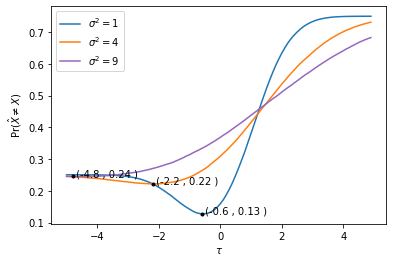
\includegraphics[width=0.4\textwidth]{solutions/ec/44/figures/fig-errorVstau}
    \caption{Plot to show Pr$ \left( \hat{X} \neq X \right)$ is minimum at negative value of $\tau$ for all nonzero values of $\sigma^2$}
    \label{ec44:fig:errorVstau}
\end{figure}
\newpage
\begin{figure}[h!]
    \centering
    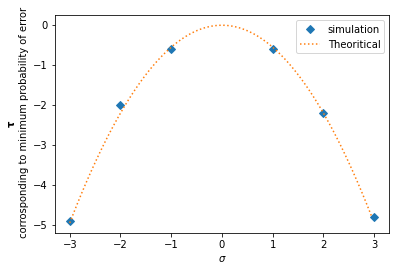
\includegraphics[width=0.4\textwidth]{solutions/ec/44/figures/fig-tauVssigma}
    \caption{Plot to show $\tau=-\frac{\sigma^2 \ln{3}}{2}$ corresponds to minimum probability of error}
    \label{ec44:fig:my_label}
\end{figure}
